\section[Windows Internals]{Windows Internals}

To understand the memory forensics of Windows, we need to understand some parts of Windows Internals, from its memory model to some kernel design. In this section we will give the reader some technical details on Windows' design.

\subsection[Memory model]{Memory model}

We start by exploring the Windows memory model. Windows by default use page size of 4KB, the address space for each process is 2GB for the 32-bit version and 8TB for the 64-bit version. The system address space is 2GB for the 32-bit version and 248TB for the 64-bit version. Every process, when run, can see its own address space and system space too, but access to system space is restricted. A typical 32-bit process can have a 2GB space for itself and a 2GB space of the system, makes a total memory space 4GB. The system space (kernel space) contains the OS and the currently running drivers. In this space contains items that specify the current state of the OS. The kernel space uses \textit{pools} to manage structures' allocation and deallocation. Windows has two types of pool, one that is \textit{pagedable} called \textit{paged pool} and the other \textit{non-paged pool}. The size of these two types of pool on Windows 10 can be reference through the table~\ref{tab:poolsize} \cite{memorylimit}. Because many parts of the OS is not used often, Windows can swap those pages out to make more space. However, critical information, including processes' information, is stored in non-paged pools.

\begin{center}
\begin{table}[h]
\begin{tabular}{|l|p{5cm}|p{5cm}|}
\hline
Pool Type & Limit on 32-bit & Limit on 64-bit \\ \hline
Paged Pool & 384 GB or system commit limit, whichever is smaller & 384 GB or system commit limit, whichever is smaller \\ \hline
Non-paged Pool & 75\% of RAM or 2 GB, whichever is smaller. & RAM or 128 GB, whichever is smaller (address space is limited to 2 x RAM) \\ \hline
\end{tabular}
\caption{Pool size on Windows 10}
\label{tab:poolsize}
\end{table}
\end{center}

The memory pool is a bitmap\footnote{An array of bits}. Windows will return the pointer and size when asked for space in the pool (chunk). Windows keeps track of chunks in the pool. At first, there is only one chunk (the pool itself). When the user asks for space, Windows will split the chunk to two, one for the user and one left unused, Windows will split the unused space in pool and return to the user for any allocation requested. Upon deallocation, Windows will merge unused chunks into one. Consider the code in Listing~\ref{lst:basicpool} for a basic example of pool allocation.

[NEED PICTURE? OR IS CODE ENOUGH]

Each chunk will have a \texttt{POOL\_HEADER} field on top to denote the content of the chunk. \texttt{POOL\_HEADER} has a size field (\texttt{BlockSize}), a previous size field (\texttt{PreviousBlockSize}), and a tag (\texttt{POOL\_TAG}). Tag is a four-byte character that Windows and Driver writer use to denote the data stored in the chunk. The typical description of \texttt{POOL\_HEADER} is at Listing~\ref{lst:poolheader}. In Table~\ref{tab:pooltag}, we listed some typical structure with its tag.

\lstinputlisting[language=C,caption={POOL\_HEADER},label={lst:poolheader},basicstyle=\linespread{0.8}]{code/poolheader.cpp}

\lstinputlisting[language=C,caption={Basic Pool Algorithm},label={lst:basicpool},basicstyle=\linespread{0.8}]{code/basic_pool.cpp}

\begin{center}
\begin{table}[h]
\begin{tabular}{|l|l|l|}
\hline
Structure     & Structure Name   & Pool Tag \\ \hline
Driver Object & \_DRIVER\_OBJECT & Driv     \\ \hline
File Object   & \_FILE\_OBJECT   & File     \\ \hline
Process       & \_EPROCESS       & Proc     \\ \hline
TCP endpoint  &                  & TcpE     \\ \hline
TCP listener  &                  & TcpL     \\ \hline
Thread        & \_ETHREAD        & Thre     \\ \hline
UDP endpoint  &                  & UdpA     \\ \hline
\end{tabular}
\caption{Some pool tag and corresponding structure}
\label{tab:pooltag}
\end{table}
\end{center}

\subsection[EPROCESS]{EPROCESS}

Windows has a special structure that contains a process information called \texttt{\_EPROCESS}. This structure is created every time when a new process spawn and located inside a non-paged pool with tag \textit{Proc}. If we have a reference to one \texttt{\_EPROCESS} we might follows \texttt{LIST\_ENTRY ActiveProcessLinks} (a doubly linked list pointer) to find other \texttt{\_EPROCESS} of different process. However because this structure can be accessed by a normal user by calling \texttt{PsLookupProcessByProcessId} one may edit the doubly linked list to remove itself from the list chain. With the given \texttt{LIST\_ENTRY} structure in \ref{lst:listentry}, refrence the graphics \ref{fig:eprocesslink} and \ref{fig:dkom} that explains the normal EPROCESS linking and modification to remove itself.

\begin{lstlisting}[language=c,caption={LIST\_ENTRY},label={lst:listentry}]
typedef struct _LIST_ENTRY {
      struct _LIST_ENTRY *Flink;
      struct _LIST_ENTRY *Blink;
} LIST_ENTRY, *PLIST_ENTRY, PRLIST_ENTRY;
\end{lstlisting}

\begin{figure}
\centering
\caption{EPROCESS Linking}
\label{fig:eprocesslink}
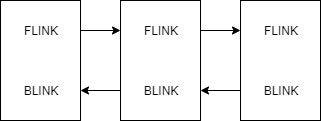
\includegraphics[]{images/eprocess_link.png}
\end{figure}

\begin{figure}
\centering
\caption{DKOM}
\label{fig:dkom}
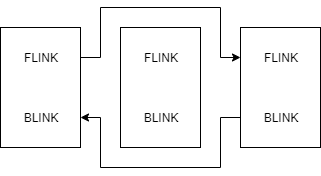
\includegraphics[]{images/dkom.png}
\end{figure}

\subsection[ETHREAD]{ETHREAD}

A process in Windows is composed by threads, for example, a process loading a library will have the library run as a thread. Every thread will have a structure in kernel to manage called \texttt{\_ETHREAD}. From an \texttt{\_ETHREAD} we can call \texttt{IoThreadToProcess} to get the parent \texttt{\_EPROCESS}, see Listing~\ref{lst:threadtoprocess}. \texttt{\_ETHREAD} allocation is also inside a non-paged pool.

\begin{lstlisting}[language=c,caption={IoThreadToProcess},label={lst:threadtoprocess}]
PEPROCESS IoThreadToProcess(
  PETHREAD Thread
);
\end{lstlisting}

\subsection[KDBG]{KDBG}

KDBG short for \texttt{Kernel Debugger Block} is one of commonly used structure when analyzing a memory artifact of Windows. It was created to easy debugging process for developers when writing OS or kernel drivers. As this struture contains pointers to others structures. One pointer contained in KDBG is \texttt{PsActiveProcessHead} which is a pointer to an \texttt{\_EPROCESS}. As previously mentioned, we can walk the list of \texttt{\_EPROCESS} to enumerate all processes.

[SHOULD THE BELOW BE PLACED SOMEWHERE ELSE?]

However from Windows 8, this structure is encoded and hinders us from analyzing windows memory. As quoted by the developers of Volatility \cite{kdbgEncoded},

\say{An encoded KDBG can have a hugely negative effect on your ability to perform memory forensics. This structure contains a lot of critical details about the system, including the pointers to the start of the lists of active processes and loaded kernel modules, the address of the PspCid handle table, the ranges for the paged and non-paged pools, etc. If all of these fields are encoded, your day becomes that much more difficult.}

While users of Volatility will suffer a bad day, Rekall's users do not as they use another method without knowledge of KDBG structure \cite{rekallOnKDBGEncoding}. However, KDBG is still an important Windows structure that provides kernel information.

\subsection[Windows dump file]{Windows dump file}

Windows provides a dump file to contains compressed memory data. This file is created by Windows when an error in kernel occur. Third party tools can dump the memory on running machine for example, DumpIt, FTK Imager. This file structure is not documented, however, it was written on Microsoft debug file, Schuster \cite{dmpfile} has written a guide to the file structure. Another dump file type is mini dump file which is documented by Joachim \cite{mdmpfile}. These dump files are commonly used to preserve the system memory state for analysis.
